\reportsection{Lean-Backed Contracts and Results}
\label{sec:results}

\subsection{Executable Interfaces} % note to be had here on language clarity: disambiguate between "proof" and "machine-checked"
\label{sec:interfaces}

The three algorithms of \cref{def:vcgeneral} are realised verbatim as a Lean~4
class, so the abstract and executable objects are the same operations;
round-trip agreement is settled by \code{native\_decide} before any security
claim is attached.
\begin{verbatim}
class VectorCommitment (V : Type) where
  Alphabet Index CommitterKey VerifierKey : Type
  Commitment CommitmentState Proof : Type
  setup  : (maxLen maxQueries : Nat) -> UInt64 -> UniversalParams
  trim   : UniversalParams -> (len queries : Nat) ->
             Prod CommitterKey VerifierKey
  commit : CommitterKey -> List Alphabet -> Prod Commitment CommitmentState
  open   : CommitterKey -> Commitment -> List Index -> ... -> Proof
  check  : VerifierKey -> Commitment -> List Index ->
             List Alphabet -> Proof -> Bool
\end{verbatim}
The transparent Merkle setup of \cref{def:vc} maps on with no secret state:
\code{setup} fixes the hash and a length bound, and \code{trim} separates the
public parameters $\pp$ into committer and verifier roles.

Hiding randomness (\cref{def:vc-hiding}) is part of this contract, not an
implementation detail.  A non-empty salt type does not by itself represent
independent salts of the required width, so the hiding interface enforces a
key-indexed randomness type, and \code{MerkleHasher} no longer exposes
\code{sampleSalt}: hiding randomness must arrive explicitly through a
\code{Randomness : CommitterKey V -> Type} field on
\code{HidingVectorCommitment}, consumed by a dedicated \code{commit\_hiding}.

\subsection{Binding: From the Experiment to the ROM Certificate}
\label{sec:binding} % binding separated from lean for now

Every ROM experiment samples one $\RO$ that the adversary, challenger, and
verifier all query (in practice the same publicly specified hash, with the same
parameters and domain separation, replaced by an ideal random function for
analysis).  Each security notion $X$ then derives its advantage from a named
experiment, $\Adv{X}(\ThetaVC):=\Pr[\Exp{X}(\adv,\ThetaVC)=1]$ over $\RO$ and
the coins, so a concrete instance cannot claim security by assigning an
arbitrary small number to an advantage field: it must pin that field to the
experiment.
Position binding (\cref{def:vc-binding}) specialises to the following
shared-oracle game.

\begin{experiment}[Merkle binding]\label{exp:binding}
Sample the shared oracle $\RO$ and derive $\pp$.  Run
\[
  (\MTCommitment,I_0,I_1,\MTMessageSubVector_0,\MTMessageSubVector_1,
    \MTProof_0,\MTProof_1)
  \leftarrow\adv^\RO(\pp).
\]
The adversary wins iff both
$\MTCheck^\RO(\MTCommitment,I_0,\MTMessageSubVector_0,\MTProof_0)$ and
$\MTCheck^\RO(\MTCommitment,I_1,\MTMessageSubVector_1,\MTProof_1)$ accept,
while $\MTMessageSubVector_0[i]\ne\MTMessageSubVector_1[i]$ for some
$i\in I_0\cap I_1$.
The budget $\querybudget$ bounds the \emph{total} number of distinct $\RO$
queries issued during the experiment, counting the adversary's queries and
the two $\MTCheck$ calls used to adjudicate the win.  This is the quantity the
birthday bound is taken over.
\end{experiment}

The win condition is captured locally by a \code{BindingBreak}: one index, two
values, and two accepted proofs.  It is the executable form of the local
witness from \cref{def:vc-binding}, not a competing definition.
\begin{verbatim}
structure BindingBreak (V : Type) [VectorCommitment V] where
  commitment : Commitment V
  index      : Index V
  value0 value1 : Alphabet V
  proof0 proof1 : Proof V

def BindingBreak.IsValid (vk : VerifierKey V) (b : BindingBreak V) : Prop :=
  Not (b.value0 = b.value1) /\
  check vk b.commitment [b.index] [b.value0] b.proof0 = true /\
  check vk b.commitment [b.index] [b.value1] b.proof1 = true
\end{verbatim}

\begin{proposition}[Binding from collision resistance]\label{thm:binding-cr}
Let $\MT[\RO]$ be a Merkle commitment whose leaf encoding is injective and
whose leaf and internal-node calls are domain separated.  If the shared
$\digestbits$-bit oracle receives at most $\querybudget$ distinct queries
during the complete experiment, then
\[
  \Adv{bind}(\ThetaVC)
  \le
  \Pr[\text{oracle-trace collision}]
  \le
  \frac{\querybudget(\querybudget-1)}{2^{\digestbits+1}}.
\]
\status{machine-checked for the shared-oracle Merkle instance}
\end{proposition}

\noindent\emph{Reason.}
A disputed index $i\in I_0\cap I_1$ yields two authentication paths that
agree at some parent but disagree below it: two distinct oracle inputs with
the same output.  The birthday bound then limits the probability of that trace
collision.

There is no hierarchy of binding definitions to traverse: the proof localises a
win in the one book-facing experiment, follows it through a disputed overlap and
two accepted paths to a trace collision, and bounds that by
$\collisionBound(\digestbits,\querybudget)$, which meets $2^{-\secpar}$ when
$\querybudget\le2^{\querybits}$ and $\secpar+1+2\querybits\le\digestbits$.

\paragraph{What is machine checked.}
\code{BindingBreak} captures the disputed-overlap step; \code{mt\_binding}
proves the colliding-paths step on a collision-free trace; the coupling theorem
bounds the trace-collision probability; and the arithmetic theorem checks the
concrete target.  These compose in the \code{HasPositionBinding MerkleVC}
instance, whose \code{binding\_bound} is
\code{win\_to\_trace\_collision.trans trace\_collision\_bound} and whose
\code{ofField} composition (\code{instantiation\_binding\_secure}, with
\code{babyBear\_binding\_secure} the BabyBear specialisation) pins the advantage
to \code{collisionBound}.  The cache extractor \code{cacheExtract\_sound}
connects accepted openings to the binding break and is recorded separately.
\status{machine-checked}

\subsection{Concrete Binding Parameters}
\label{sec:params}

The digest and salt widths are not chosen by hand.  The derivation of
$(D,k,S)$ from $(\field,\secpar,h)$ stated in \cref{sec:attack} is realised as
the \code{ofField} constructor of \code{MerkleHasherParams}.  The predicate
\code{MeetsBindingTarget p} ($\secpar+1+2h\le\kappa$, where $\kappa=b\cdot D$)
is decidable, and \code{meetsBindingTarget\_ofField} proves it holds for every
output of \code{ofField}; \code{MeetsFieldSaltTarget} and
\code{MeetsByteSaltTarget} certify the salt-space cardinality prerequisite for
hiding.

\paragraph{Certificates are generated, not enumerated.}
For any field, target, and query budget, one operation derives the parameters
through \code{of\_field}, checks the binding margin and salt cardinality, and
either returns a certificate carrying the proved bounds or refuses the claim.
Each obligation is explicit and all four are closed here: the deterministic
theorem assumes away collisions, the birthday theorem knows nothing about Merkle
openings, a reduction without a shared-oracle verifier never connects trace to
acceptance, and an abstract bound without a parameter rule never fixes how many
field elements a digest must contain.

\begin{finding}[BabyBear binding certificate]\label{finding:capstone}
Let $b=30$ (conservative BabyBear field-element bits), $\secpar=128$, and
$h=64$.  Then \code{ofField 30 128 64} produces
\[
  D=9,\qquad \kappa=270\text{ bits},\qquad k=5,\qquad S=16.
\]
The binding margin is
$270-(128+1+2\cdot64)=13$ bits.  Thus the nine-element digest satisfies the
side condition of \cref{thm:binding-cr} for $q\le2^{64}$ and carries the
fully proven ROM binding certificate.
\status{proved; \texttt{native\_decide} + arithmetic theorem}
\end{finding}

The one-element digest ($D=1$, $\kappa=30$) from \cref{sec:motivation} and
the certified $D=9$ digest are two points on the same rule; the former cannot
inherit the theorem because it does not satisfy the arithmetic premise.

\begin{table}[H]
  \centering
  \caption{BabyBear parameters at $\secpar=128$, $h=64$, computed by
    \code{MerkleHasherParams.ofField 30 128 64} and verified by
    \texttt{native\_decide}.  Salt widths $k$, $S$ are proved cardinality
    certificates; the Merkle ROM hiding theorem is the next composition
    milestone.}
  \label{tab:babybear}
  \begin{tabular}{@{}lccccl@{}}
    \toprule
    Configuration & $D$ & $\kappa$ (bits) & $k$ & $S$ (bytes) & Binding status \\
    \midrule
    Single field element ($D=1$) & $1$ & $30$ & --- & --- & \baseline{refused} \\
    \code{ofField 30 128 64}
      & \ours{\textbf{9}} & \ours{\textbf{270}}
      & \ours{\textbf{5}} & \ours{\textbf{16}}
      & \ours{\textbf{machine-checked}} \\
    \bottomrule
  \end{tabular}
\end{table}


\subsection{Hiding: From the Root Contract to the Selective-Opening Target}
\label{sec:hiding}

The hiding interface (\cref{sec:interfaces}) names the distributional
obligation a Merkle instance must discharge.  It encodes root hiding
(\cref{def:root-hiding}) as a bound on \code{PMF.etvDist} between the real and
ideal root games, and carries the theorem field that the selective-opening
target (\cref{def:selective-hiding}) will eventually fill.
\begin{verbatim}
class HasROMHiding (V : Type) [VectorCommitment V] where
  Hidden        : Type
  rootRealGame  : PMF Hidden
  rootIdealGame : PMF Hidden
  rootError privacyError : ENNReal
  root_hiding :
    PMF.etvDist rootRealGame rootIdealGame <= rootError
\end{verbatim}

\begin{proposition}[Hiding from unqueried salted inputs]\label{thm:hiding-rom}
Consider a Merkle commitment with $\msglen$ independently sampled
$\saltbits$-bit leaf salts, injective fixed-width leaf encodings, and one
shared random oracle.  A root-hiding distinguisher can gain information only
through a bad event: it queries a hidden salted leaf input, or it encounters an
internal-hash collision during the root hybrid.  Consequently, the intended
ROM bound has the form
\[
  \Adv{hide}(\ThetaVC)
  \le
  \frac{\msglen\querybudget}{2^{\saltbits}}
  + \varepsilon_{\mathrm{internal}}(\digestbits,\querybudget,\shape).
\]
\status{intended Merkle ROM reduction; composition target}
\end{proposition}

\noindent\emph{Reason.}
If no hidden salted input was queried and the internal hybrid encounters no
collision, replacing the hidden leaf labels and root with fresh oracle outputs
does not change the adversary's view.  A successful distinguisher must trigger
one of those bad events.

\paragraph{What is machine checked.}
The artefact supplies the support for \code{HasROMHiding}: typed hiding
randomness, structural root-hiding lemmas, total-variation distance, a negative
theorem for deterministic salts, and salt-cardinality capstones.  Discharging
\code{root\_hiding} and lifting it to the selective-opening target
(\cref{def:selective-hiding})---an oracle-native leaf argument, a bottom-up root
hybrid, and a simulator for the full disclosed view---is the next composition
step; the proved salt sizes are prerequisites for it, not a completed theorem.

\begin{finding}[Hiding foundation]\label{finding:hiding}
For BabyBear at $\secpar=128$,
\code{babyBear\_byte\_salt\_hiding} and
\code{babyBear\_field\_salt\_hiding} prove that $S=16$ byte salts and $k=5$
field salts each define a space of at least $2^{128}$ elements.  The
operational interface consumes explicit typed randomness, and the structural
root-hiding foundation is represented in Lean.
\status{machine-checked foundation; ROM composition next}
\end{finding}

\subsection{Measured Cost of the Security Contracts}

The parameter rules identify which configurations support the intended claims;
the benchmark sweeps show what they cost.  Each plot fixes a binary tree with
$4{,}096$ leaves and $32$ openings and reports Criterion means for prover time
(\code{commit}$+$\code{open}), verifier time (\code{check}), and proof size,
with field-coloured vertical lines at the first configuration reaching
$\lambda\ge128$ (and $\lambda\ge256$ where present) and a red \textsf{x} at each
level transition.  We report the Poseidon2 sweeps, where the field dependence is
sharpest; the Bytewise Blake3 sweeps state the same decisions in bytes ($S=16$
salt and $32$-byte digest for $\lambda\ge128$), stepping at compression-block
rather than permutation boundaries.

\paragraph{Field dependence.}
The Poseidon2 hiding sweep (top) reaches the $\secpar=128$ cardinality threshold
at $k=5$ for BabyBear, $k=3$ for Goldilocks, and $k=1$ for BN254; the binding
sweep (bottom) reaches $\lambda\ge128$ at $D=9$, $D=5$, and $D=2$ respectively.
Both are direct consequences of field capacity.  Proof size grows continuously
with each added salt or digest element; runtime steps only at the red
\textsf{x} markers.

\begin{figure}[H]
  \centering
  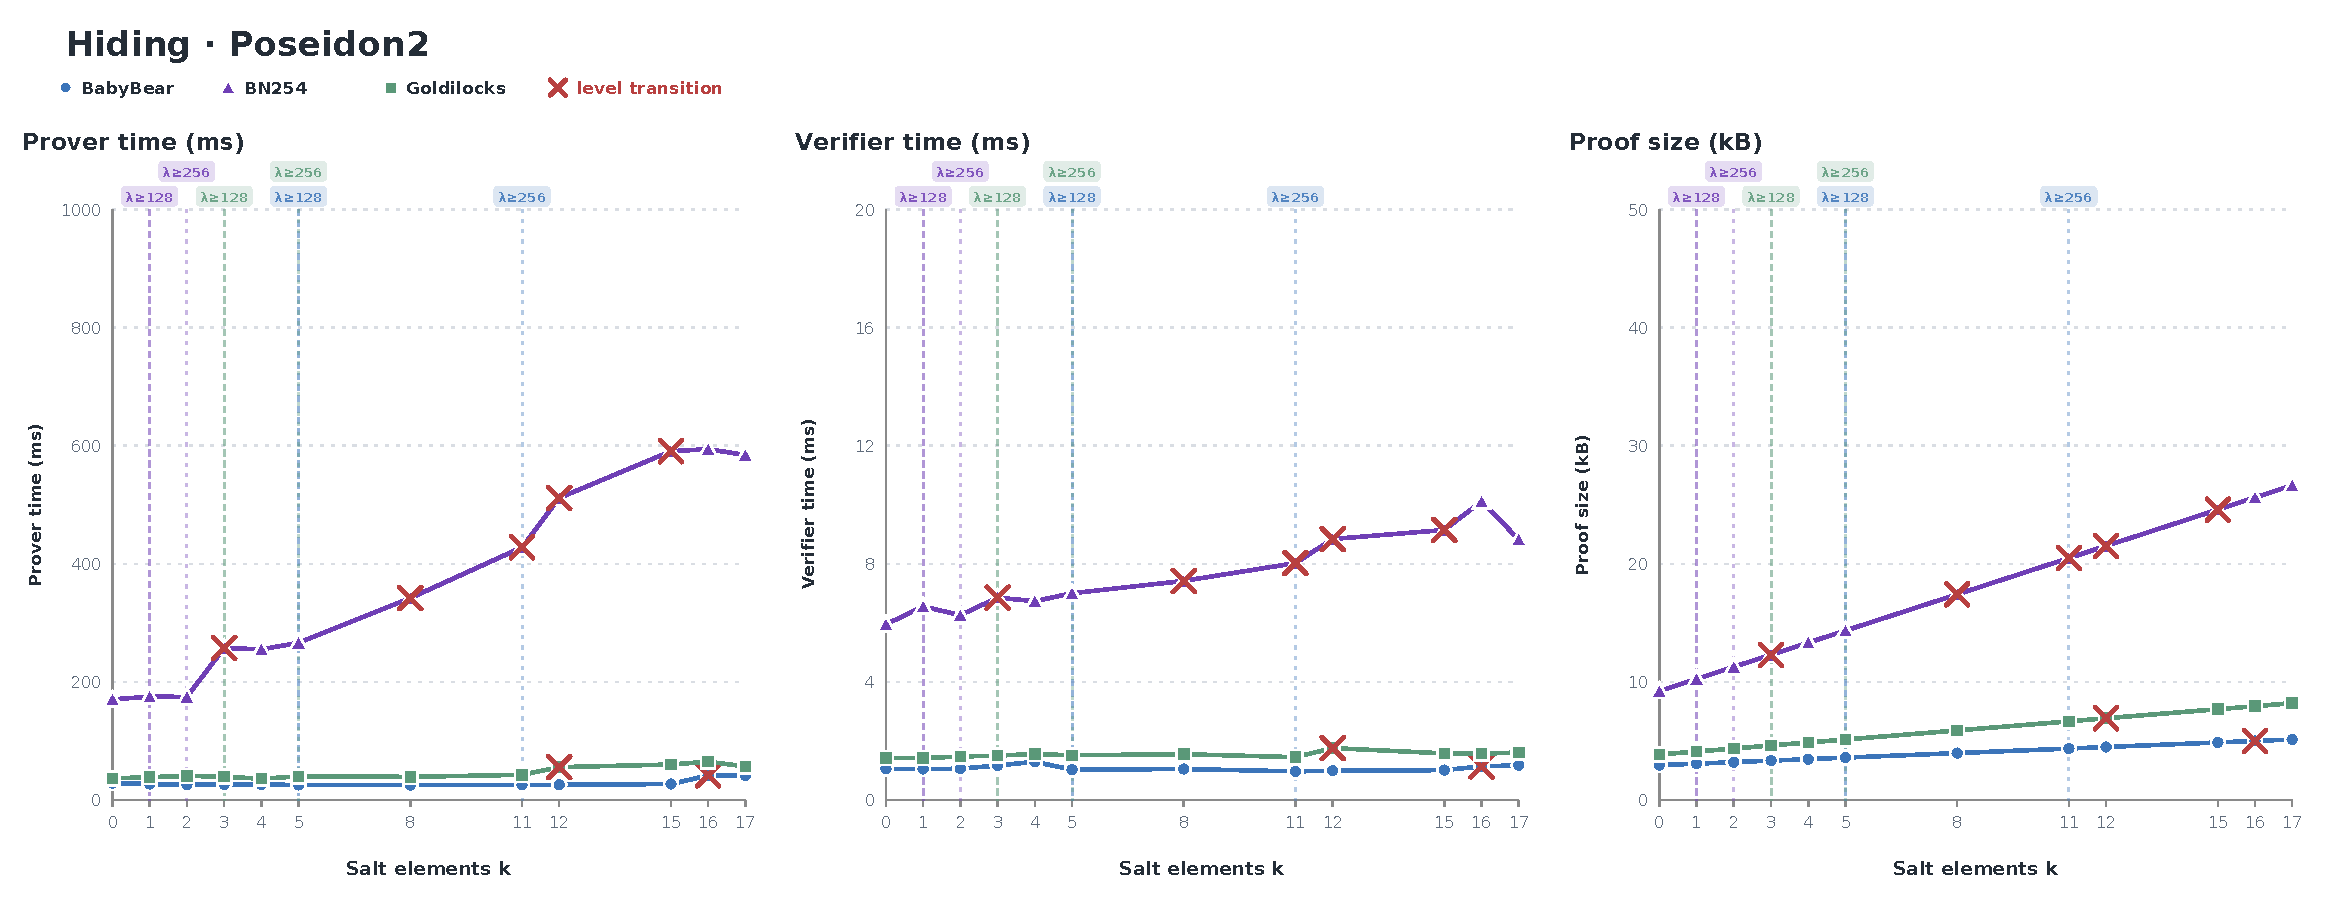
\includegraphics[width=0.65\textwidth]{figures/benchmark_hiding_poseidon_triptych_extra_x.pdf}\\[0.3em]
  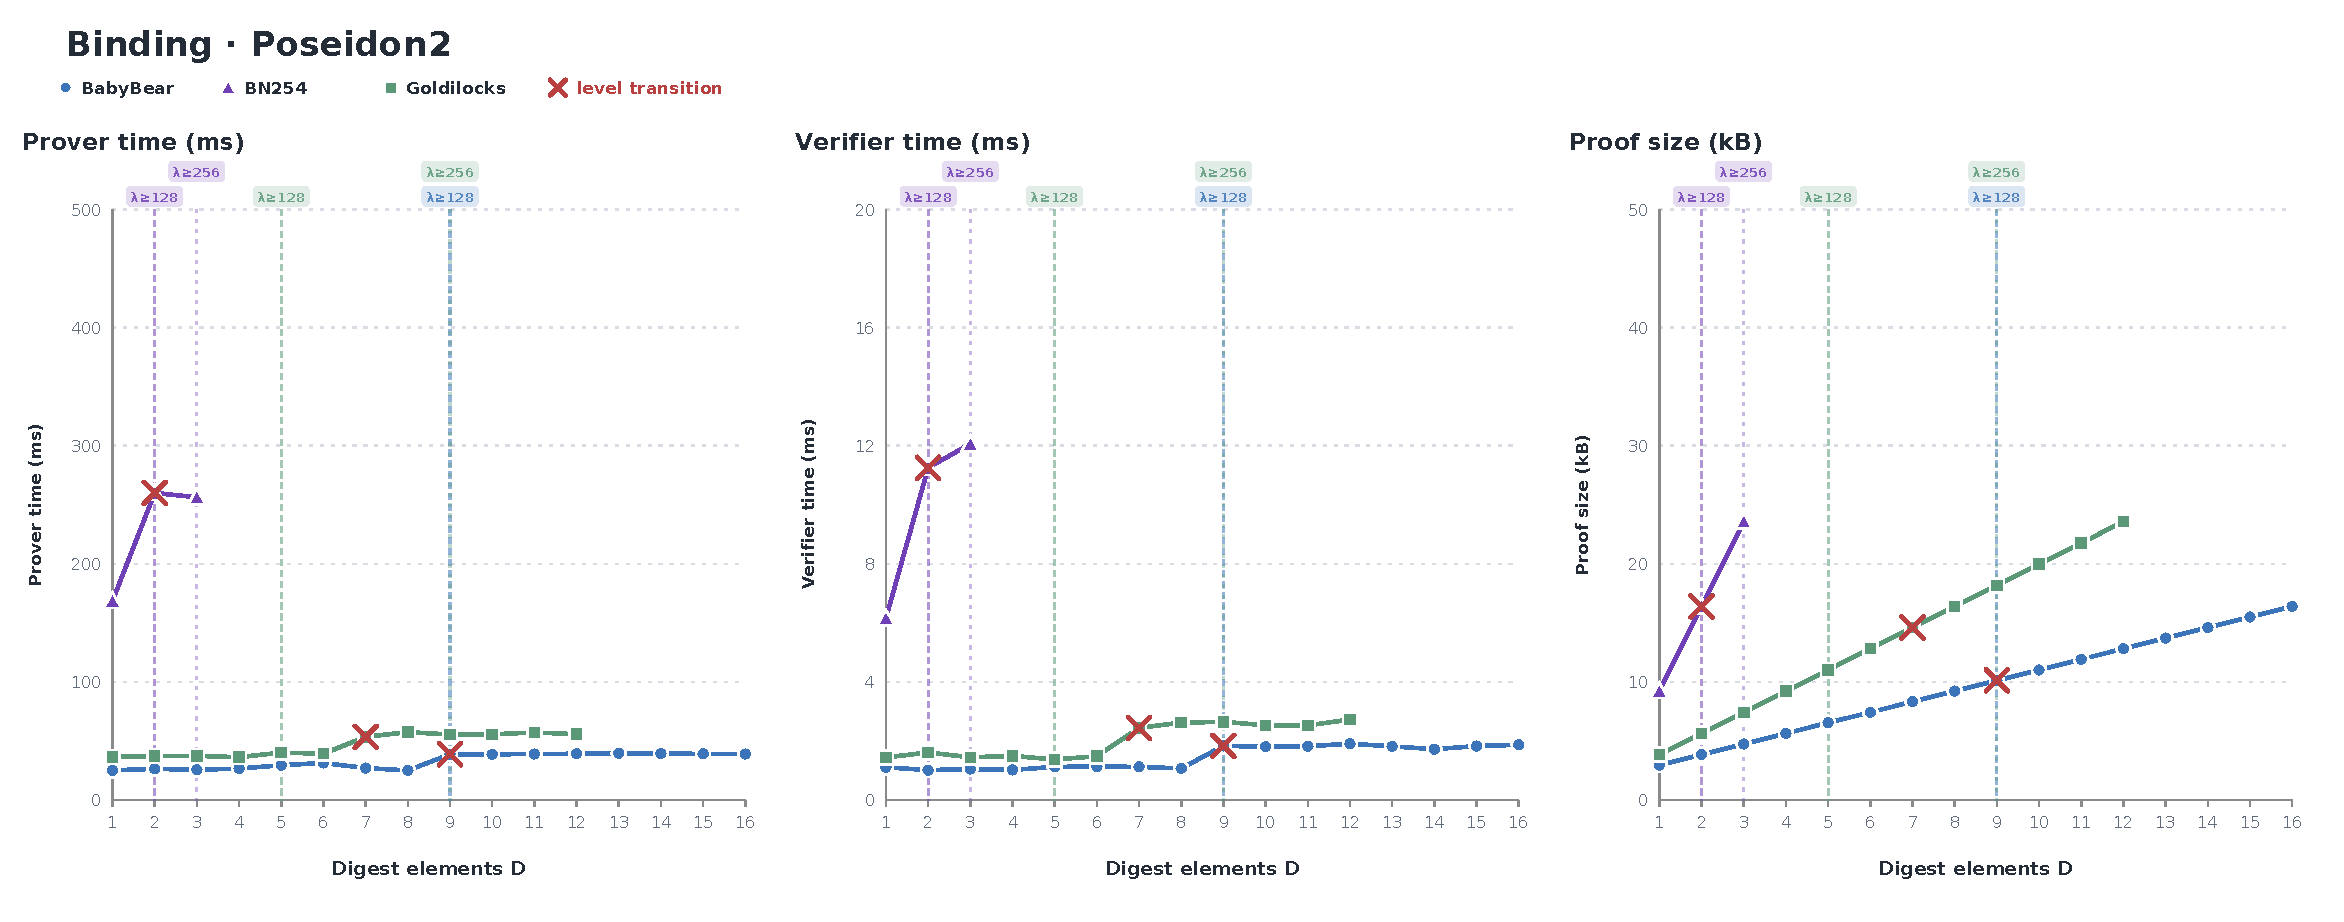
\includegraphics[width=0.65\textwidth]{figures/benchmark_binding_poseidon_triptych_extra_x.pdf}
  \caption{Poseidon2 hiding cost as salt width grows (top) and binding cost as
  digest width grows (bottom).  Field-coloured vertical lines mark the first
  measured $\lambda\ge128$ and $\lambda\ge256$ configurations for BabyBear,
  Goldilocks, and BN254; red \textsf{x} markers identify inputs that cross into
  an additional permutation.}
  \label{fig:poseidon-cost}
\end{figure}

The security threshold and the cost transition are different events, so both
must be inspected.  For Poseidon2 both the $\lambda\ge128$ and $\lambda\ge256$
thresholds land \emph{before} the first red \textsf{x} for all three fields:
the certified parameters sit inside the permutation block Poseidon2 has already
computed for its rate-width output, so correct security is algebraically free at
these levels.  Across the Bytewise Blake3 sweeps only the $128$-bit hiding salt
($S=16$) clears before its first compression-block transition, while $256$-bit
hiding ($S=32$) and the $128$- and $256$-bit binding digests ($32$ and $64$
bytes) all land on a red \textsf{x}, so there the security upgrade and the extra
Blake3 compression block arrive together rather than for free.
\status{empirical; binary tree with $4{,}096$ leaves and $32$ openings}

\reportsection{Conclusion}{The spine turns a security target into a proved,
priced contract for any compliant \textsf{ark-mt} instantiation.} % future work section maybe instead
\label{sec:conclusion}

A vector commitment is only as strong as the parameters underneath it, and the
default \textsf{ark-mt} configurations miss that target for small fields on both
axes at once.  We fix the boundary at the level of the reference, recover the
Merkle tree as its instantiation, and turn each obligation into an executable,
Lean-checked contract: binding is closed end to end, while the hiding interface
and cardinality certificates are in place for the remaining ROM composition.  A
designer supplies $(\field,\secpar,H)$ and an interface choice and receives the
derived parameters with the evidence that they meet the target; the same
framework extends to new fields and hashes without starting over.
